\documentclass[a4paper,14pt]{extarticle}

\usepackage[a4paper,top=20mm,bottom=20mm,left=30mm,right=10mm]{geometry}
\usepackage[T1,T2A]{fontenc}
\usepackage[utf8]{inputenc}
\usepackage[russian]{babel}
\usepackage{indentfirst}
\usepackage{titlesec}
\usepackage{graphicx}
\usepackage{listings}

\renewcommand{\baselinestretch}{1.3}
\titleformat{\section}{\normalsize\bfseries}{\thesection}{1em}{}
\titleformat{\subsection}{\normalsize\bfseries}{\thesection}{1em}{}
\setlength{\parindent}{12.5mm}

\begin{document}
	
	\newpage\thispagestyle{empty}
	\begin{center}
		\MakeUppercase{
			Министерство науки и высшего образования Российской Федерации\\
			Федеральное государственное бюджетное образовательное учреждение высшего образования\\
			<<Вятский Государственный Университет>>\\
		}
		Институт математики и информационных систем\\
		Факультет автоматики и вычислительной техники\\
		Кафедра электронных вычислительных машин
	\end{center}
	\vfill
	
	\begin{center}
		Отчет по лабораторной работе №4\\
		по дисциплине\\
		<<Информатика>>\\
		<<Форматы представления числовой информации.\\Представление целых чисел>>
	\end{center}
	\vfill
	
	\noindent
	\begin{tabular}{ll}
		Выполнил студент гр. ИВТб-1301-05-00 \hspace{5mm} &
		\rule[-1mm]{25mm}{0.10mm}\,/Макаров С.А./\\
		
		Руководитель доцент кафедры ЭВМ & \rule[-1mm]{25mm}{0.10mm}\,/Коржавина А.С./\\
	\end{tabular}
	
	\vfill
	\begin{center}
		Киров 2024
	\end{center}
	
	\newpage
	\section*{Цель}
	Цель лабораторной работы: закрепить на практике знания форматах представления числовой информации. Написать программы, решающие описанные ниже задачи. Программы должны работать без ошибок на любых наборах входных данных.
	
	\section*{Задание}
	\begin{enumerate}
		\item Представить беззнаковое (неотрицательное) число в n-разрядной сетке. На входе через пробел: целое число в десятичной системе счисления, разрядность сетки. На выходе: строка, отображающая введенное число в разрядной сетке.
		
		\item  Представить число в прямом коде в n-разрядной сетке. На входе через пробел: целое число в десятичной системе счисления, разрядность сетки. На выходе: строка, отображающая введенное число в прямом коде.
		
		\item Представить число в дополнительном коде в n-разрядной сетке. На входе: целое число в десятичной системе счисления, разрядность сетки. На выходе: строка, отображающая введенное число в дополнительном коде.
		
		\item Представить число в обратном коде в n-разрядной сетке. На входе: целое число в десятичной системе счисления, разрядность сетки. На выходе: строка, отображающая введенное число в обратном коде.
		
		\item Определить расстояние по Хеммингу двух дополнительных кодов. Расстояние по Хеммингу -- количество знакопозиций, в которых отличаются два кода, например, для кода Грея расстояние по Хеммингу между соседними кодами равно 1. На входе: два целых числа в десятичной системе счисления, разрядность сетки. На выходе: число -- расстояние по Хеммингу между ДК введенных чисел.
	\end{enumerate}
	
	\section*{Решение}
	\subsection*{Задание 1}
	Схема алгоритма для решения предлагаемой задачи представлена на рисунке 1.

	\begin{figure}[h]
		\centering
		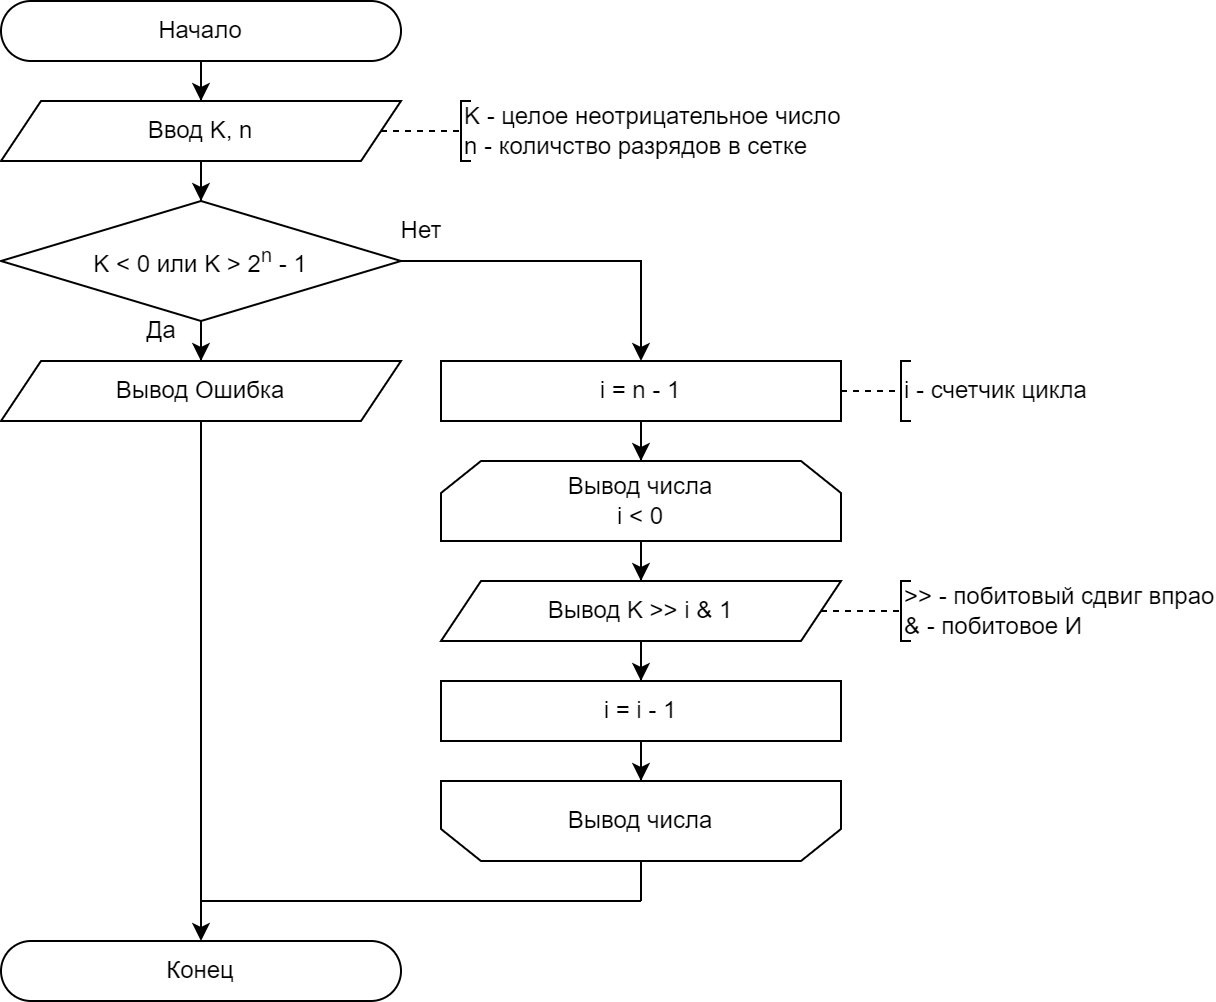
\includegraphics[width=0.8\linewidth]{schemes/s-1}
	\end{figure}
	\begin{center}
		Рисунок 1 – Схема алгоритма задания 1
	\end{center}
	
	Решение задачи на языке C представлено ниже.
	
	\begin{lstlisting}[tabsize=2,basicstyle=\ttfamily]
#include <stdio.h>
#include <math.h>
int main() {
	int K, n;
	scanf("%d %d", &K, &n);
	if (K < 0 || K > pow(2, n) - 1) {
		printf("Error");
		return 0;
	}
	
	for (int i = n - 1; i >= 0; i--) {
		printf("%d", K >> i & 1);
	}
	return 0;
}
	\end{lstlisting}
	
	\subsection*{Задание 2}
	Схема алгоритма для решения предлагаемой задачи представлена на рисунке 2.
	
	\begin{figure}[h]
		\centering
		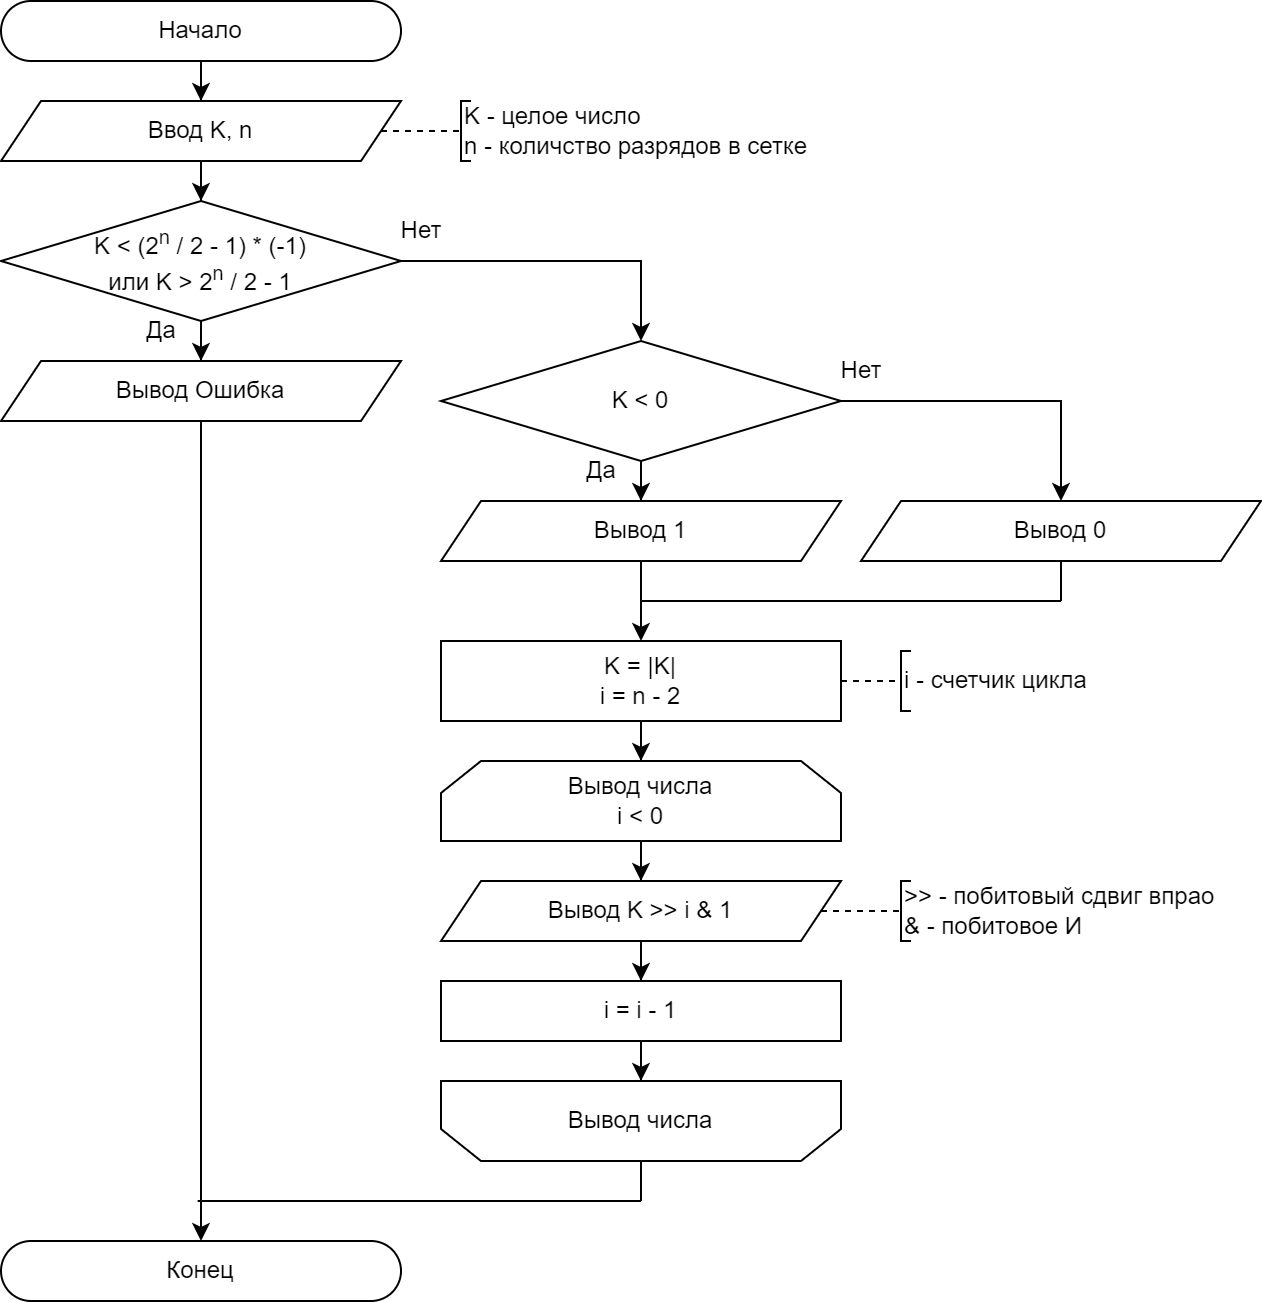
\includegraphics[width=0.8\linewidth]{schemes/s-2}
	\end{figure}
	\begin{center}
		Рисунок 2 – Схема алгоритма задания 2
	\end{center}
	\pagebreak
	
	Решение задачи на языке C представлено ниже.
	
	\begin{lstlisting}[tabsize=2,basicstyle=\ttfamily]
#include <stdio.h>
#include <math.h>
int main() {
	int K, n;
	scanf("%d %d", &K, &n);
	if (K > pow(2, n) / 2 - 1 
			|| K < (pow(2, n) / 2 - 1) * -1) {
		printf("Error");
		return 0;
	}
	printf("%d", K < 0 ? 1 : 0);
	K = abs(K);
	for (int i = n - 2; i >= 0; i--) {
		printf("%d", K >> i & 1);
	}
	return 0;
}
	\end{lstlisting}
	
	\pagebreak
	\subsection*{Задание 3}
	Схема алгоритма для решения предлагаемой задачи представлена на рисунке 3.
	
	\begin{figure}[h]
		\centering
		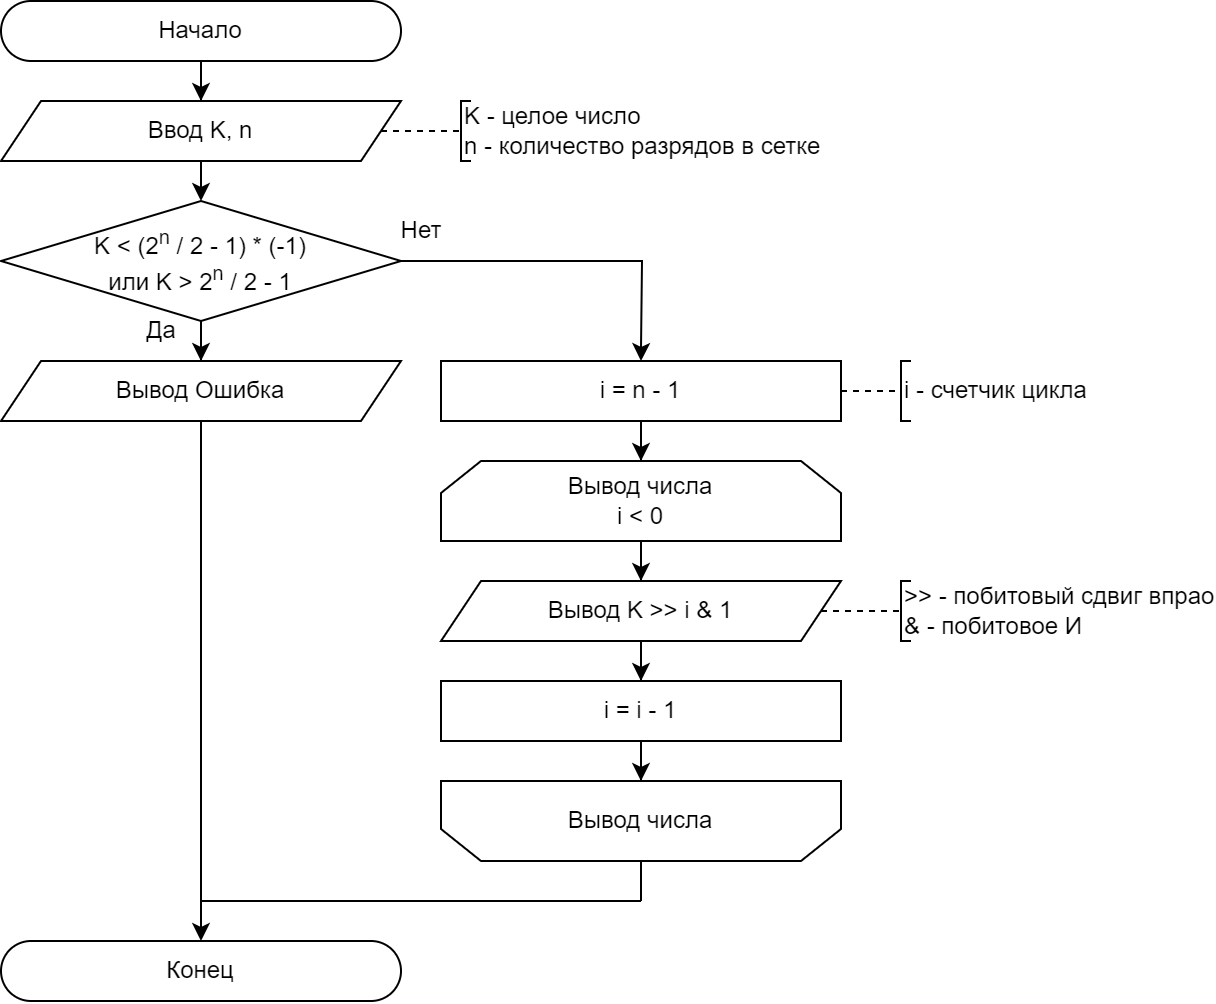
\includegraphics[width=0.8\linewidth]{schemes/s-3}
	\end{figure}
	\begin{center}
		Рисунок 3 – Схема алгоритма задания 3
	\end{center}
	
	Решение задачи на языке C представлено ниже.
	
	\begin{lstlisting}[tabsize=2,basicstyle=\ttfamily]
#include <stdio.h>
#include <math.h>
int main() {
	int K, n;
	scanf("%d %d", &K, &n);
	if (K > pow(2, n) / 2 - 1 
			|| K < pow(2, n) / 2 * -1) {
		printf("Error");
		return 0;
	}
	for (int i = n - 1; i >= 0; i--) {
		printf("%d", K >> i & 1);
	}
	return 0;
}
	\end{lstlisting}
	
	\subsection*{Задание 4}
	Схема алгоритма для решения предлагаемой задачи представлена на рисунке 4.
	
	\begin{figure}[h]
		\centering
		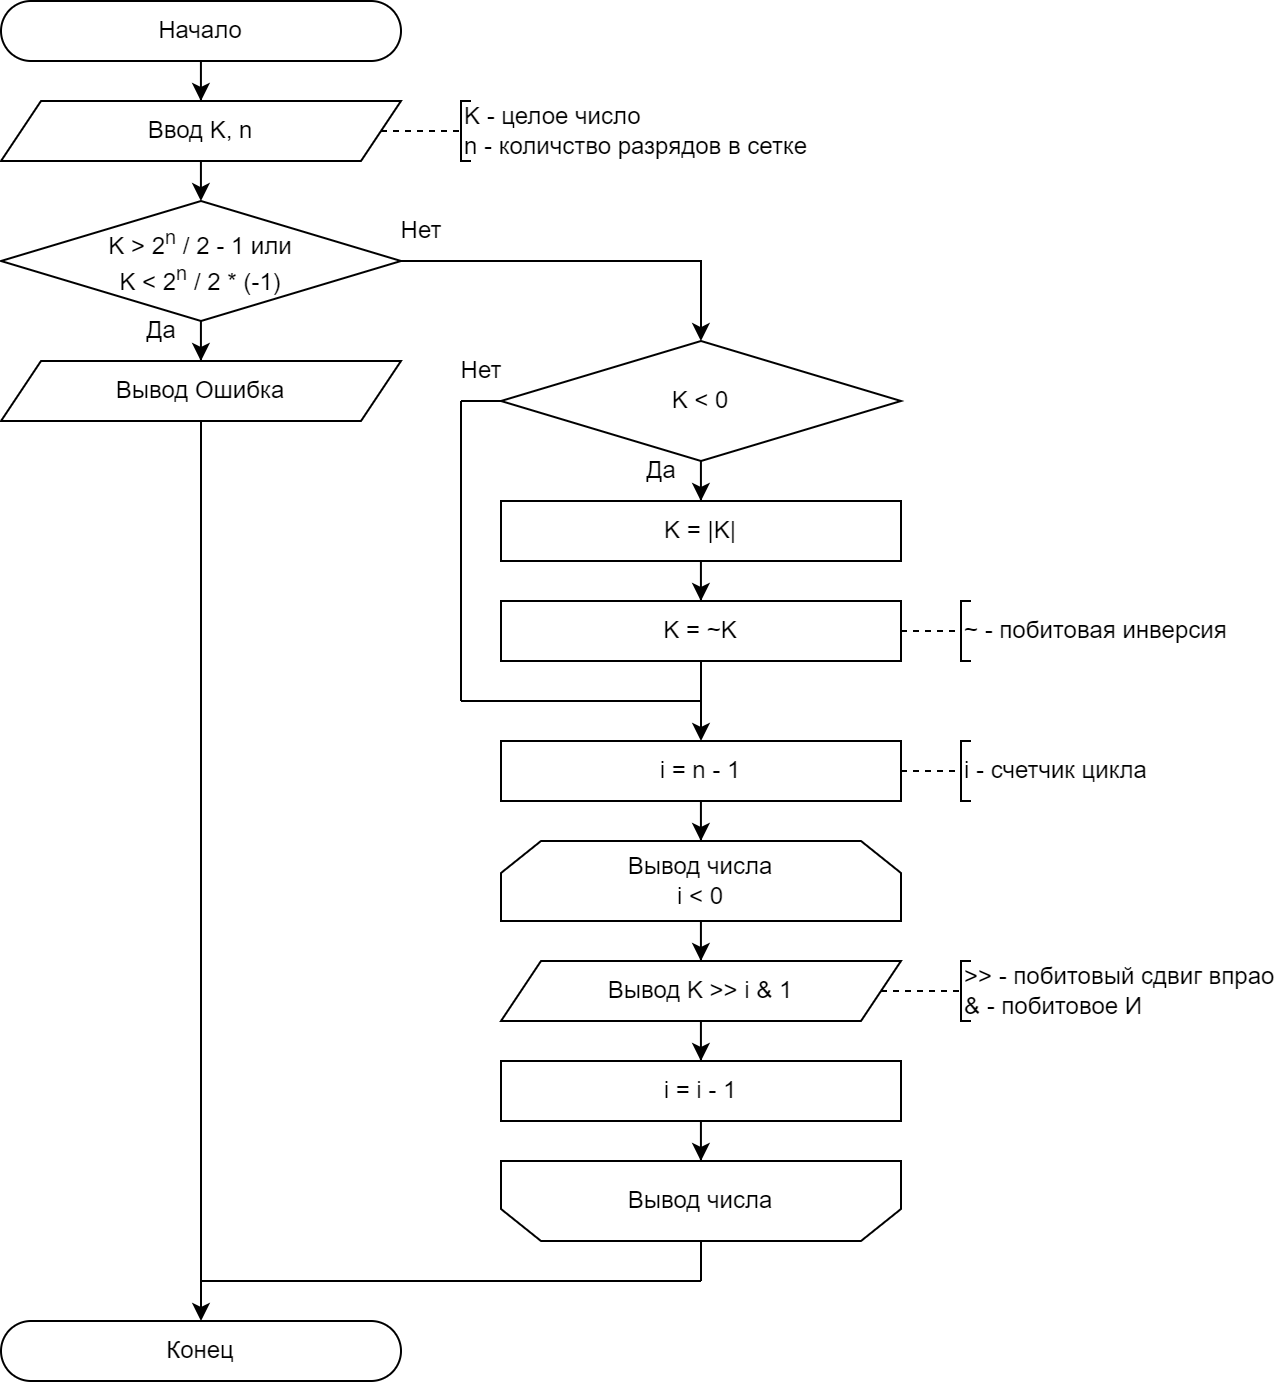
\includegraphics[width=0.8\linewidth]{schemes/s-4}
	\end{figure}
	\begin{center}
		Рисунок 4 – Схема алгоритма задания 4
	\end{center}
	\pagebreak
	
	Решение задачи на языке C представлено ниже.
	
	\begin{lstlisting}[tabsize=2,basicstyle=\ttfamily]
#include <stdio.h>
#include <math.h>
int main() {
	int K, n;
	scanf("%d %d", &K, &n);
	if (K > pow(2, n) / 2 - 1 
			|| K < (pow(2, n) / 2 - 1) * -1) {
		printf("Error");
		return 0;
	}
	if (K < 0) {
		K = abs(K);
		K = ~K;
	}
	for (int i = n - 1; i >= 0; i--) {
		printf("%d", K >> i & 1);
	}
	return 0;
}
	\end{lstlisting}
	
	\pagebreak
	\subsection*{Задание 5}
	Схема алгоритма для решения предлагаемой задачи представлена на рисунке 5.
	
	\begin{figure}[h]
		\centering
		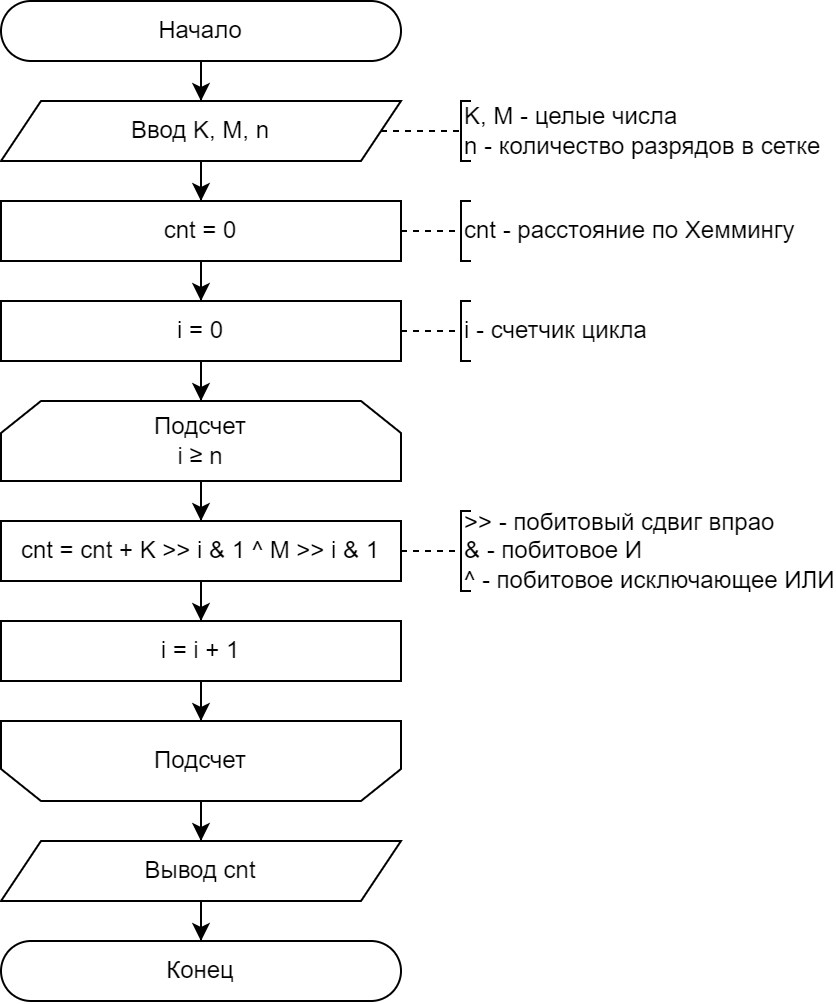
\includegraphics[width=0.6\linewidth]{schemes/s-5}
	\end{figure}
	\begin{center}
		Рисунок 5 – Схема алгоритма задания 5
	\end{center}
	
	Решение задачи на языке C представлено ниже.
	
	\begin{lstlisting}[tabsize=2,basicstyle=\ttfamily]
#include <stdio.h>
int main() {
	int K, M, n;
	scanf("%d %d %d", &K, &M, &n);
	int cnt = 0;
	for (int i = 0; i < n; i++) {
		cnt += K >> i & 1 ^ M >> i & 1;
	}
	printf("%d", cnt);
	return 0;
}
	\end{lstlisting}
	
	\section*{Вывод}
	В ходе выполнения лабораторной работы удалось закрепить на практике знания использования различных систем счисления, реализовав алгоритмы работы с целыми и вещественными числами в различных системах счисления.
	
\end{document}